\chapter{Chapter 2 : Change-point detection state of the art}\label{chp:2}

\minitoc

As discussed in Chapter \ref{chp:1}, it is critical to determine time periods during which the properties of the concentration signal are constant. This is a mathematical problem that has been extensively addressed in the literature in the form of breakpoint detection. There are two types of breakpoint detection algorithms:

\begin{itemize}
\item \textbf{Off-line methods:} There are numerous reviews of this topic in the literature, among the most extensive are \cite{basseville1993detection,truong2020}. In these methods, one works with the entire data signal. Breakpoints are identified by following the signal from the most recent date to the earliest date. There are numerous applications of these methods in different application areas \cite{chen2012parametric,levy2009detection,Shi2022,Li2021}
\item \textbf{On-line methods:} a detailed description of these methods can be found in \cite{basseville1993detection}. The difference with the methods of the previous point is that the detection of a breakpoint is done when the data is read. The goal is to detect as quickly as possible a point in time during the reading where the characteristics of the signal have changed. 
\end{itemize}

This work will focus only on the off-line methods that we will develop in the following sections. This choice was motivated by the operational speed of data samplng and storing on which this work is based. Clearly, on-line detection methods would be of interest to the Anses if the goal were to act urgently and investigate any potentially anomalous signal as soon as it is detected. However, the agency's missions are longer term in nature. At the time this work began, data were being collected annually, so the use of online methods was inappropriate. Nevertheless, for readers who wish to refer to it, we can state that there is no shortage of online detection methods in the literature \cite{liu2017change,Li2021,hohle2010online,ranganathan2010pliss,li2015m}.

Breakpoint detection methods were excluded from this work and therefore are not be presented in this state of the art. Although these methods are of interest to the task set in this manuscript. The focus of this work was to explore frequentist models and their adaptation to the specificities of concentration data (see Chapter \ref{chp:3}). However, numerous examples of application of bayesian methods can be found in the literature \cite{rigaill2012exact,tartakovsky2010state,adams2007bayesian,zhao2010bayesian,liang2019using}.

The outline of the state of the art is strongly based on the nomenclature established in (Truong). Section 1 describes the modelling used in the theory of breakpoint detection theory in parametric and nonparametric frameworks will be described in Section 1. The breakpoint search methods are then discussed in Section 2. The various existing methods for calibrating the penalty for the case where the number of breaks is unknown are presented in Section 3. Although the bulk of our work deals with univariate data, we will extend the methods discussed to the case where the variables are multivariate.


\section{Models}\label{chp2:model}

Several terms are introduced and will be retained in this section. We consider a signal consisting of observations $\bm y = (y_1,...,y_n)$ which are the realisations of random variables $Y_1,...,Y_n$. This signal is assumed to be piecewise stationary and univariate. Its properties are constant over parts, which we will call segments, and change at times $t_1^* <... < t_k^* <... < t_{K^*}^*$. A segment of the signal from the u-th coordinate to the v-th is noted $y_{u:v}$. Following the convention, let $t_0 = 0$ and $t_{K^*+1} = n$. In our context, the purpose of breakpoint detection is to estimate the positions $t_k^*$ and the number of breaks $K^*$ when it is unknown. 

The search for a segmentation $\mathcal{T}_{K^*}$  of a signal $\bm y$ into $K^*+1$ segments can be formally described as an optimization problem. More precisely, one tries to minimise a quantitative criterion. Without loss of generality, the criterion chosen in our case corresponds to a cost $\mathcal{C}(\mathcal{T},\bm y)$ and, more precisely, to the sum of the cost of each segment defined by $\mathcal{T}_{K^*}$: 
\begin{equation}\label{chp:2:cost}
\mathcal{C}(\mathcal{T}_{K^*},\bm y) = \sum_{k=0}^{K^*} W(y_{t^*_k+1:t^*_{k+1}}),
\end{equation}
where $W(y_{t^*_k+1:t^*_{k+1}})$ denotes the cost of the kth segment. The ultimate goal is to find the segmentation that minimizes \ref{chp:2:cost}. The function chosen to model the cost of a segment $W$ determines the types of changes detected. Its choice can also depend on whether a parametric of non parametric settings is desirable. 
It is assumed that $K^*$ is always assumed to be unknown. It will sometimes be necessary to assume that $K^*$ is known in order to introduce certain algorithms. In this case, it is explicitly stated that this will be the case. the knowledge of the number of breakpoints change the optimization problem. In the case, where $K^*$ is known the problem consists in solving: 
\begin{equation}\label{chp:2:optKnown}
\min_{\lvert\mathcal{T}\rvert = K^*} \mathcal{C}(\mathcal{T},\bm y), 
\end{equation}     
It transforms to a penalized optimization problem when $K^*$ is unknown: 
\begin{equation}\label{chp:2:optnKnown}
\min_{\mathcal{T}} \{ \mathcal{C}(\mathcal{T},\bm y) + pen(\mathcal{T}) \} 
\end{equation}      


\subsection{Parametric setting}\label{chp2:sec:likm}

In the parametric case, the detection depends heavily on what we are looking for in the signal $\bm y$. For example, searching for slope changes in a signal \cite{Bai1994,Fearnhead2018} does not require the same modelling as detecting changes in the mean \cite{Frick2014,chen2012parametric}. We restrict our investigation to a cost function based on maximum likelihood. In this setting, the observations located in the $k$-th segment is supposed to be following a distribution $Q$ depending on a set of parameters $\bm \theta_k$. More formally, we have that:
$$y_t \sim f(.;\bm \theta_k)\mathbbm{1}_{t_{k}^*+1\leq t \leq t_{k+1}^*},$$
with $f$ being the density function of distribution $Q$. In other words, we suppose that all observations emanate from the same distribution $Q$ but the values of $\bm \theta_k$ change abruptly at each change-point $t^*_k$. We supppose that $\bm \theta \in \Theta$ with $\Theta$ being a subset of $\mathbb{R}^d$ and compact. 
The cost function used to evaluate segments in this context is the negative log-likelihood. Hence, for a segment $y_{u:v}$ with $u < v$, we can write:  
$$W(y_{u:v}) = -\sup_{\bm \theta \in \Theta} \sum_{i = u}^{v} \ln f(y_i; \bm \theta)$$ 

In this case, the optimization problem \ref{chp:2:optnKnown} rewrites as: 
\begin{equation}\label{chp:2:penlik}
\min_{\mathcal{T} = (t_0 < t_1 < ... < t_K < t_{K+1})} \{ -\sup_{\bm \theta \in \Theta} \sum_{k=0}^K \sum_{i = t_k+1}^{t_{k+1}} \ln f(y_i; \bm \theta_k) + pen(\mathcal{T}) \} 
\end{equation}       

These models are very common in litterature and were adapted to various types of distributions $Q$. The investigations spread from the gaussian, to distribution belonging to the exponential family and even to discrete distribution. 

\subsection{Non-Parametric setting}\label{chp2:sec:multrank}

The cost function for a segment can also be adapted for nonparametric statistical inference. Several strategies have been developed in the literature over time. These include the nonparametric maximum likelihood method \cite{Zou2014,Einmahl2003}, kernel methods \cite{Harchaoui2008,li2015m}, and rank-based methods \cite{Pettitt1980,Wang2019}. We will focus on the latter here for two main reasons. First, the ranked based methods were already known from the experts working with the Anses. Second, the method we are presenting here can be adapted for left-censored observations.  

Detecting a breakpoint in a signal can be done using a test statistic based on the ranks of the observations rather than their values. The rank of the ith observation is defined as $R_i = \sum_{j =1}^n\mathbbm{1}(X_j < X_i)$. Moreover, we note $\hat{F}_n(t) = \frac{1}{n}\sum_{i = 1}^n\mathbbm{1}(X_i < t)$ the empirical cumulative distribution function (c.d.f.). The cost function is derived from the Wilcoxon/Mann-Whitney rank criterion. This is equivalent to running the test under the following assumptions: 
\begin{itemize}
  \item $\mathcal{H}_0$: there are no breaks in the $\bm Y = (Y_1,...,Y_n)$ 
  \item $\mathcal{H}_1$: there is a change $t^*$ such that $Y_1,...,Y_{t^*}$ are distributed according $\mathbb{P}_1$ and $Y_{t^*+1},...,Y_{n}$ are distributed according to $\mathbb{P}_2$. 
\end{itemize}
The rank statistic of the $t$-th observation is centered and is written as follows:
\begin{equation}\label{chp2:statranknp}
  U_n(t) = \frac{2}{\sqrt{nt(n-t)}}\sum_{i = 1}^{t}\bigg(\frac{n+1}{2} - R_i\bigg)
\end{equation}
The test statistic for $\mathcal{H}_0$ and $\mathcal{H}_1$ is defined as:
\begin{equation}\label{chp2:stattestnp}
  S_n(t) = \hat{\Sigma}_n^{-1} U^2_n(t),
\end{equation}
where $\hat{\Sigma}_n = \frac{4}{n}\sum_{i=1}^n(\hat{F}_n(X_i)-1/2)^2$. Theorem 1 of \cite{lung2015} shows that under the null hypothesis the $S_n$ are distributed according to a $\chi^2$ distribution.

The non parametric test statistic was extended to multiple changepoint detection by \cite{lung2015}. The cost function $W$ for a segment $y_{u:v}$ is defined as: 
\begin{equation}
  W(y_{u:v}) = -(v-u)\hat{\Sigma}^{-1}_n\overline{R}^2_{u:v},
\end{equation}
where $\overline{R}_{u:v} = \frac{1}{v-u}\sum_{i = u}^vR_i$ is the average rank of $y_{u:v}$.

In this case, the optimization problem \ref{chp:2:optKnown} rewrites as: 
\begin{equation}\label{chp:2:npcost}
\min_{\lvert\mathcal{T}\rvert = K}  -\sum_{k=0}^K \sum_{i = t_k+1}^{t_{k+1}} (t_k+1-t_{k+1})\hat{\Sigma}^{-1}_n\overline{R}^2_{t_k+1:t_{k+1}}
\end{equation}       

\section{Searching for change points}

Various methods for finding breakpoints have been described in the literature. They can be distinguished according to whether they provide an optimal solution to the problems \ref{chp:2:optKnown} and \ref{chp:2:optnKnown} or an answer in the form of an approximation. Only the optimal methods are listed here. Approximation methods are not discussed, but there are plenty of them, such as sliding window methods \cite{Li2010,Liu2022}, bottom-up segmentation \cite{chen1998speaker}, and binary segmentation \cite{Yang2001,Fryzlewicz2014}. Two methods that provide an optimal solution are presented below.

\subsection{Optimal segmentation approach}\label{chp2:opt}

The optimal segmentation algorithm brings an answer to problem \ref{chp:2:optKnown}. With a fixed $K$ number of change-points, one can recursivly solve the optimization problem. The recursion comes from the following relationship: 
\begin{equation}\label{chp2:recurs}
\min_{\lvert\mathcal{T}\rvert = K}\mathcal{C}(\mathcal{T},\bm y) = \min_{t \leq n-K}\{W(y_{1:t})+\min_{\lvert\mathcal{T}\rvert = K-1}\mathcal{C}(\mathcal{T}, y_{t:n})\} 
\end{equation}
In other words, given all possible segmentations of all sub-signals $y_{t:n}$ in $K-1$ segments, one can compute the optimal segmentation of the whole signal $\bm y$ in $K$ segments. This results in a computationnal cost in order of $\mathcal{O}(Kn^2)$ \cite{haynes2017}. Algorithm \ref{chp2:algo:opt} shows the implementation of \ref{chp2:recurs}. 


\begin{algorithm}[ht]
\caption{Optimal partition algorithm:}\label{chp2:algo:opt}
\begin{algorithmic}

\State \textbf{input} : signal $y_{1:n}$, cost function $W()$, number of changepoints $K \geq 1$
\State Create $C_1$ a $n\times n$ empty matrix
\ForAll{$(u,v)$ such that $1 \leq u < v \leq n$}
  \State $C(u,v) \gets W(y_{u:v})$
\EndFor
\If{$K+1 > 2$}
  \For{$k = 2,...,K$}
    \ForAll{$u,v \in \{1,..,n\}$ such that $v-u > k$}
      \State $C_k(u,v) \gets \min_{u+k-1 \leq t < v} C_{k-1}(u,t) + C_1(t+1,v)$ 
    \EndFor
  \EndFor
\EndIf
\State $L \gets (0,...,0)$ vector of size $K+1$
\State $L{K+1} \gets n$
\State $k \gets K+1$
\While{$k > 1$}
  \State $s \gets L(k)$
  \State $t^* \gets \arg\min_{k-1\leq t < s}C_{k-1}(1,t)+C_1(t+1,s)$
  \State $L(k-1) \gets t^*$
  \State $k \gets k-1$
\EndWhile
\State \textbf{Output:} a list $L$ of $K$ estimated changepoints (with $n$ as a last coordinate).
\end{algorithmic}
\end{algorithm} 

Appplication of this optimal partitionning methods can be found in \cite{rigaill2015pruned,Lavielle1997,perron2006dealing}

\subsection{PELT algorithm}\label{chp2:pelt}

The Pruned Exact Linear Time (PELT) algorithm solves problem \ref{chp:2:optnKnown}. It was introduced by \cite{Killick2012}. It has a computationnal in order of $\mathcal{O}(n)$ when the penalty term $pen(\mathcal{T})$ is linear in the number of change points e.g. $pen(\mathcal{T}) = \beta K$ where $\beta > 0$ is the addtionnal cost one must pay each time a break is decided in the signal $\bm y$. The pruning rule can be stated as follows: \\
for $t<s < n$, if
\begin{equation}\label{chp2:pruning}
 \min_{\mathcal{T}}\bigg[\mathcal{C}(\mathcal{T},y_{0:t})+\beta\lvert \mathcal{T}\rvert\bigg] + W(y_{t+1:s}) \geq \min_{\mathcal{T}}\bigg[\mathcal{C}(\mathcal{T},y_{0:s})+\beta\lvert \mathcal{T}\rvert\bigg], 
\end{equation}
holds, then $t$ can never be the last changepoint prior to $n$.   
One can sequentially go through the signal $\bm y = \{y_s\}_{s=1}^n$ and obtain a set of potential breakpoints $\{t_0,...,t_k\}$ for each index $s \in {1,...,n}$. Then, one should proceed to eliminate candidates from this set using this pruning rule. This is the principle of Algorithm \ref{chp2:algo:pelt}.

\begin{algorithm}[ht]
\caption{PELT algorithm}\label{chp2:algo:pelt}
\begin{algorithmic}

\State \textbf{input} : the data $y_{1},...,y_{n}$, a cost function $W()$, and the penalty term $\beta_{n}$ \\
  
\State \textbf{initialisations} : $F(0)=-\beta_{n}$, $R_{1}=\lbrace 0\rbrace$, $CP(0)=NULL$  
  
\ForAll{$\tilde t=1,...,n$} :
  \State Compute 
  $ F(\tilde t)=\min_{t\in R_{\tilde t}}\lbrace F(t)+W(y_{(t+1):\tilde t})+\beta_{n}\rbrace $
  \State Compute $ \overline t=\arg \min_{t\in R_{\tilde t}}\lbrace F(t)+W(y_{(t+1):\tilde t})+\beta_{n}\rbrace $ 
  \State Set $CP(\tilde t)=[CP(\overline t), \overline t]$
  \State Set $R_{\tilde t+1}=\left\{t\in R_{\tilde t}\cup \lbrace\tilde t\rbrace \vert F(t)+W(y_{(t+1):\tilde t}) +\beta_{n} \le F(\tilde t)   \right\}$ 
\EndFor 
   
\State \textbf{output} : the vector of change-points $CP$. 
 
\end{algorithmic}
\end{algorithm} 

This method is very popular in litterature, one can find numerous examples in very diverse fields \cite{Wang2015,Wang2021,Kosta2015}.

\section{Estimation of the number of changes}\label{chp2:nb_change}

This section propose diverse methods to estimate the number of changes $K$ in $\bm y$. In the case of using a penalized criterion e.g. \ref{chp:2:optnKnown}, this is equivalent of tuning the penalty term. This state of the art deals only deals with linear penalties as mentionned in \ref{chp2:pelt}. They take the form $pen(\mathcal{T}) = \beta K$ with $\beta > 0$. Other types we will not discuss in this work (see for instance \cite{Harchaoui2010,Zhang2006,NIPS2010}). When no penalized criterion is used, there are other methods for selecting the best segmentation. 

\subsection{Different heuristics}\label{chp2:pencal}

\subsubsection{Methods for penalty calibration}

The solution of problem \ref{chp:2:optnKnown} depends on the penalty value $\beta$. The choice of this value can be viewed as a model selection problem. The higher the penalty value, the lower the number of fractions and therefore the higher the segmentation cost. There are many procedures for calibrating the value of $\beta$. We describe here only those that were used in this work: 

\begin{itemize}
  \item The BIC criterion: this is one of the most popular procedures in the literature for change point detection and more generally for model selection. It is applied in the case of parametric modelling. In the context of break detection, this criterion is written as follows: $pen(\mathcal{T}) = \frac{p}{2}\log(n)$ where $p$ represents the dimension of the parameters $\bm \theta$. Examples of the BIC criterion use can be found in \cite{YAO1988181,faure2016comparison,Shi2022}. As stated in \cite{faure2016comparison} fixing the penalty term parameter $\beta$ \textit{a priori} is not suited for the data at hand. In our case, the BIC led to overestimate the number of change points in all experiments. We can say that it didn't scale to our types of data. A more data driven calibration method was needed.    
  \item The slope heuristic: Sometimes it is necessary to use other methods to calibrate the penalties. It can be stated that the BIC is appropriate when the modelling is parametric. It depends on the dimension of the parameter $\bm \theta$ so it is hardly applicable when the inference is non-parametric inference. The slope heuristic \cite{Birge2006} allows us to solve this problem and, in particular, to determine a minimal value of the penalty $\beta_{min}$. If we plot the successive values of $\mathcal{C}_k$ for different $k$ with respect as a function of $\beta$, we obtain a decreasing curve. The values of $\mathcal{C}_k$ for high values of $k$ have a linear behaviour. We can define the minimum penalty value $\beta_{min}$ as the slope of this line. Moreover, the ideal value of the penalty is at the value $2\beta_{min}$. This procedure has been used on various applications \cite{Baudry2011,Bardet2012,arlot2009data}.
\end{itemize}

Other methods can be cited like the Akaike Information Criterion or the dimension jump.  

\subsubsection{Methods using the optimal partitioning algorithm}

Although Optimal Partition Algorithm \ref{chp2:algo:opt} is used to solve the problem in 2.1 and therefore requires a fixed number of $K+1$ segments to work, the number of segments can also be estimated as follows. Assuming that the actual number of interruptions is less than a number $K_{max}$, Algorithm \ref{chp2:algo:opt} should be run for a number of breaks $K$ between 1 and $K_{max}$. We can then plot the cost of the $K_{max}$ different segments obtained according to the number of breaks. 

The curve is divided into two parts. The first part shows the cost decreasing rapidly with the number of change points, with a much smaller decrease in cost above a certain number of breaks $\hat{K}$ \cite{LAVIELLE20051501}. It is precisely this value $\hat{K}$ that we choose as the estimator for the number of change points. To capture this value automatically, a elbow method is used. One can find other examples of the elbow method in \cite{liu2020determine,syakur2018integration}. It is also used in the \textit{Multrank} detection method \cite{lung2015} as it obtains the best results for the estimation of $K^*$.

We can give an \texttt{R} based algorithm of the elbow method in Algorithm \ref{chp2:algo:elbow}. We note $\mathcal{C}_k$ the cost of the optimal segmentation of signal $\bm y$ in $k+1$ segments. This can be done using basic \texttt{R} functions like the linear model function \texttt{lm}:   

\begin{algorithm}[ht]
\caption{Elbow method algorithm}\label{chp2:algo:elbow}
\begin{algorithmic}

\State \textbf{input} : the segmentations cost $\mathcal{C}_k$ for $k \in \{1,...,K_{max}\}$ \\

\State \textbf{initialisations} : Initialize $C \gets (\mathcal{C}_1,...,\mathcal{C}_{K_{max}})$, \\
Initialize $slope \gets (0,...,0)$  a $K_{max}-2$ length vector. 
\For{$k = 2,...,K_{max}-1$}
  \State $ml1 \gets \texttt{lm}(C(1:k) \sim 1:k)$
  \State $ml2 \gets \texttt{lm}(C(k:K_{max}) \sim k:K_{max})$
  \State $slope(k-1) \gets \sum ml1\$ residuals + \sum ml2\$ residuals$
\EndFor
\State $CP \gets (2:K_{max}-1)(which.min(slope))$
\State \textbf{output} : the optimal number of changes $CP$. 
 
\end{algorithmic}
\end{algorithm} 

\subsection{Exploratory approach: CROPS algorithm}

The methods of calibration of the penalty value of the problem \ref{optnknown}, allow to set $\beta$ to a certain and ideal value. The algorithm CROPS: Changepoints for a Range Of PenaltieS algorithm defines a more exploratory approach. It allows to search a range of penalties $[\beta_{min},\beta_{max}]$ and to find the penalty values wihtin that range associated with new segmentations.  

The proccess to uncover new penalty values $\beta \in [\beta_{min},\beta_{max}]$ is based on theorem 3 of \cite{haynes2017}. Noting $U_k(y_{i:n}) = \min_{\mathcal{T}_k} \sum_{j = 0}^k W(y _{t_j+1:t_{j+1}})$ the unpenalized cost of the optimal segmentation in $k$ changepoints of $\bm y$ and $m(\beta)$ the number of changepoints of the optimal segmentation result obtained usng $\beta$ in problem \ref{chp:2:optnKnown}, the theorem writes as follows:

\begin{theorem}
Let $\beta_0 < \beta_1$, 3 cases are possible to uncover new penalty values:
\begin{enumerate}
  \item If $m(\beta_0) = m(\beta_1)$ then $m(\beta) = m(\beta_0)$ for all $\beta \in [\beta_0,\beta_1]$
  \item If $m(\beta_0) = m(\beta_1)+1$ then $m(\beta) = m(\beta_0)$ for all $\beta\in[\beta_0,\beta_{int}[$ and $m(\beta) = m(\beta_1)$ for all $\beta\in[\beta_{int},\beta_1]$ with:
  \begin{equation}\label{chp2:crit:crops}
    \beta_{int} = \frac{U_{m(\beta_1)}(y_{1:n})-U_{m(\beta_0)}(y_{1:n})}{m(\beta_0)-m(\beta_1)}
  \end{equation}
  \item If $m(\beta_0) > m(\beta_1)+1$ and $m(\beta_{int}) = m(\beta_1)$ where $\beta_{int}$ is defined in \ref{chp2:crit:crops}, then $m(\beta) = m(\beta_0)$ if $\beta\in[\beta_0,\beta_{int}[$ and $m(\beta) = m(\beta_1)$ if $\beta\in [\beta_{int},\beta_1]$
\end{enumerate}
\end{theorem} 

From this theorem is derived the CROPS Algorithm \ref{chp2:algo:crops}.  

\begin{algorithm}[ht]
\caption{CROPS algorithm}\label{chp2:algo:crops}
\begin{algorithmic}

\State \textbf{input} : the data $y_{1},...,y_{n}$, \\
the bounds of the initial interval of penalties $\beta_{min}$ and $\beta_{max}$, \\
\texttt{PELT} algorithm 
  
\State Compute \texttt{PELT}$(y_{1:n},\beta_{min})$ and \texttt{PELT}$(y_{1:n},\beta_{max})$ 
\State Define $\beta^* \gets \{(\beta_{min},\beta_{max})\}$ a list of vectors.  
\While{$\beta^*\neq \emptyset$}
  \State Define $(\beta_0, \beta_1) \gets \beta^*(1)$
  \If{$m(\beta_0) > m(\beta_1)+1$}
    \State $\beta_{int} \gets \frac{\mathcal{Q}_{m(\beta_1)}(y_{1:n})-\mathcal{Q}_{m(\beta_0)}(y_{1:n})}{m(\beta_0)-m(\beta_1)}$
    \State $res \gets$ \texttt{PELT}$(y_{1:n},\beta_{int})$
    \State From $res$ store $m(\beta_{int})$
    \If{$m(\beta_{int})\neq m(\beta_1)$}
      \State $\beta^* \gets \{\beta^*,(\beta_0,\beta_{int}),(\beta_{int},\beta_1)\}$
    \EndIf
  \EndIf
  \State $\beta^* \gets \beta^*$\textbackslash$(\beta_0,\beta_1)$
\EndWhile 
   
\State \textbf{output} : Detailed segmentation for all $\beta \in [\beta_{min},\beta_{max}]$. 
\end{algorithmic}
\end{algorithm} 

An estimation of the number of changes can be obtained by combining the results of Algorithm  \ref{chp2:algo:crops} with the elbow method. For each $\beta$ uncovered by CROPS, we have the number of changes $m(\beta)$ and the cost $\mathcal{C}_{\beta}(\bm y_{1:n})$. We can run Algorithm \ref{chp2:algo:elbow} to estimate an optimal number of changes. Keeping the results of other segmentations found by CROPS for exploratory purposes. 

\section{Extension to the multivariate case}

In the Section \ref{chp2:model}, it was stated that the $\bm y$ signal is univariate. It is possible to extend the methods for detecting breaks to the multivariate case. It is now assumed that the variables are $y_i = (y_i^1,...,y_i^D)$ where $D$ is the dimension of the individual observations. Two types of settings for multivariate cahnge points are highlighted in \cite{pickering2016changepoint}. Both of them are illustrated in Figure \ref{fig:multicp}:

\begin{itemize}
  \item Fully multivariate methods: If a breakpoint is determined in the signal $\bm y$, then this break is then present in the $D$ dimensions. 
  \item Multivariate subset methods: If a breakpoint is determined in the signal $\bm y$, then this break is only present only in a subset of the $D$ dimensions.
\end{itemize}

\begin{figure}[ht]
  \centering
  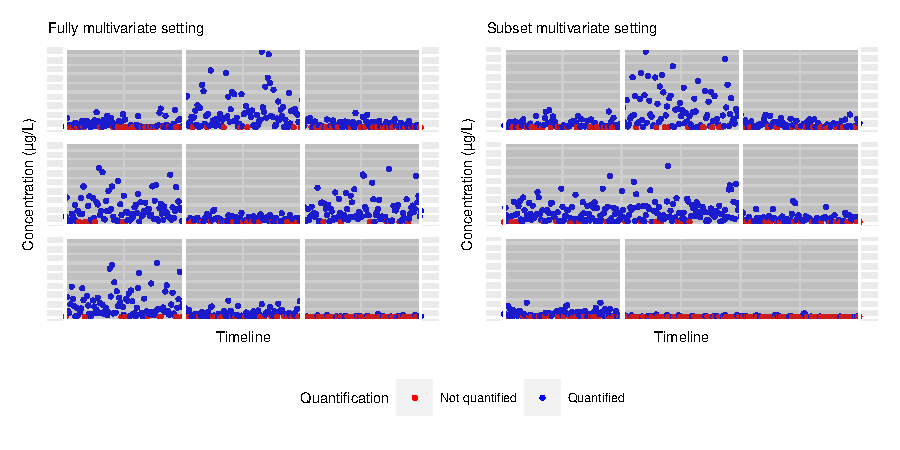
\includegraphics[]{figs/Chap2/MultiCP.pdf}
  \caption{Two examples showing the difference between fully and subset multivariate settings.}
  \label{fig:multicp}
\end{figure}

Most models presented in this section \ref{chp2:model} are extensible to the multivariate case and lead to fully multivariate methods. For example, parametric models can be fitted by using multivariate likelihood, see . The penalized likelihood criterion \ref{chp:2:penlik} is always used to solve Problem \ref{chp:2:optnKnown}. The choice of penalty values is still made with procedures as in \ref{chp2:pencal}. In the non paramétrique case, the \textit{Multrank} method can also be extended to multivariate settings. This necessits a to adapt \ref{chp:2:npcost} as:  

\begin{equation}\label{chp:2:npcostmulti}
\min_{\lvert\mathcal{T}\rvert = K}  -\sum_{k=0}^K \sum_{i = t_k+1}^{t_{k+1}} (t_k+1-t_{k+1})\overline{\bm R}'_{t_k+1:t_{k+1}}\bigg(\hat{\Sigma}_n^D\bigg)^{-1}\overline{\bm R}_{t_k+1:t_{k+1}},
\end{equation}       
where $\overline{\bm R}_{u:v} = (\overline{R}^{(d)}_{u:v})_{d=1}^D$, $\overline{R}^{(d)}_{u:v}$ is the average rank of the segment defined by $u$ and $v$ of the $d$-th dimension $y^{(d)}_{u:v}$, and $\hat{\Sigma}_n^D$ is the $D$-dimensionnal empirical covariance matrix. 

The crucial point leading to fully multivariate detection is that the assumption that there are change points in the signal $\bm y$ does not take into account that only certain variables may be affected. To overcome this problem and thus create multivariate subset methods, it is assumed in \cite{pickering2016changepoint} that the change-points locations $(t_0,...,t_{K+1})$ are associated with subsets of variables $(\mathcal{S}_0,...,\mathcal{S}_{K+1})$. A subset $\mathcal{S}_k$ indicates which variables among the $D$ changed. For each times in the series $t \in [1:n]$, we can define a vector of change points $c^t = (c_1^t,...,c_D^t)$ where $c_d^t$ is the last change point position known prior to instant $t$ for variable $d$ including $t$. At the time changes $t_k$, we have that $c_d^{t_k} = t_k$ if $d \in \mathcal{S}_k$. The size of subset $\mathcal{S}_k$ is noted $q_{t_k} = \sum_{d=1}^D\mathbbm{1}(c_d^{t_k} = t_k)$. Denoting, $W_d(y_{u:v})$ the cost of segment $u:v$ for the $d$-th variable, \cite{pickering2016changepoint} derived a penalized criterion similar to \ref{chp:2:optnKnown} to minimize: 

\begin{equation}\label{chp:2:optnKnownmulti}
\mathcal{C}(\mathcal{T},\bm y) + pen(\mathcal{T}) = \sum_{k = 0}^{K+1}\bigg(\sum_{d=1}^D \bigg[ q_{t_k}W_d(y_{(c^{t_k}_d+1):c^{t_{k+1}}_d})\bigg] + pen(q_{t_k}) \bigg) + pen(\mathcal{T})
\end{equation}      

We can see that this criterion bears two penalty terms. $pen(\mathcal{T})$ was already discussed in Section \ref{chp2:nb_change} and serves the purpose of not overestimate the number of changes $K$. $pen(q_{t_k})$ avoids the over estimation of the number of variables in subset $\mathcal{S}_k$. 




